% !TeX root = 00_main.tex

\chapter[Introduction]{Introduction}

It is estimated that a third of the 130 billion copies of applications distributed by Apple's App Store\textsuperscript{\textregistered} access a user's geographic location \cite{appledownloads,appslocation}. As an example, the recently launched augmented reality game ``Pok\'emon Go'', which has been downloaded more than 100 million times on Android devices alone \cite{pokemongo}, constantly synchronizes the GPS location of users with a company server. While users trust that their location data will be used in sensitive fashion, Apple\textregistered{} recently updated its privacy policy to allow sharing the spatio-temporal location of their users with ``partners and licensees''\cite{appleprivacy}.

The mobility behavior of a person often reveals a large variety of sensitive information, which they may not be aware of.
A list of potentially sensitive professional and personal information that could be inferred about an individual, knowing only their mobility trace, was published recently by the Electronic Frontier Foundation \cite{Blumberg2009}. Such personal information could simply be marketing information, obtained from a user's choice of restaurants, or a user's religious beliefs, inferred through the proximity to a particular church. It can also indicate other, much more sensitive, information about an individual based on their presence in a motel or at a medical clinic.

\begin{figure}[p]
	\centering
	\begin{subfigure}[b]{\textwidth}
		\centering
		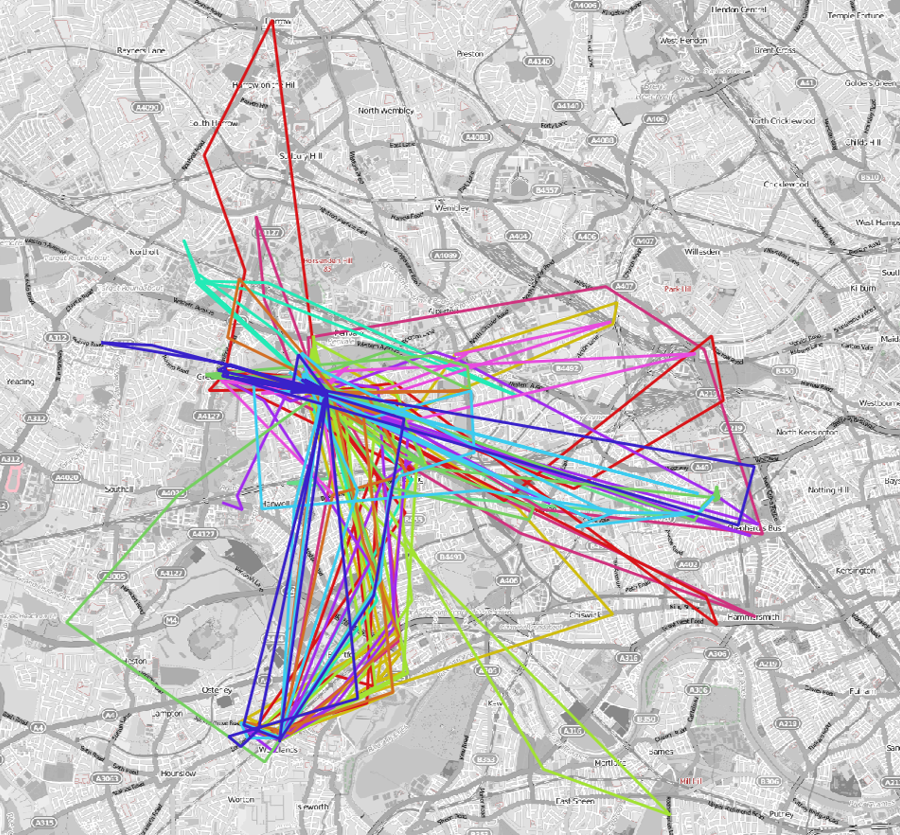
\includegraphics[width = 0.7\textwidth]{figures/1_user_12_week_small.png}
		\subcaption{Weekly history of a single user.}
    \label{fig:intro:1user}
  \end{subfigure}

	\begin{subfigure}[b]{\textwidth}
		\centering
		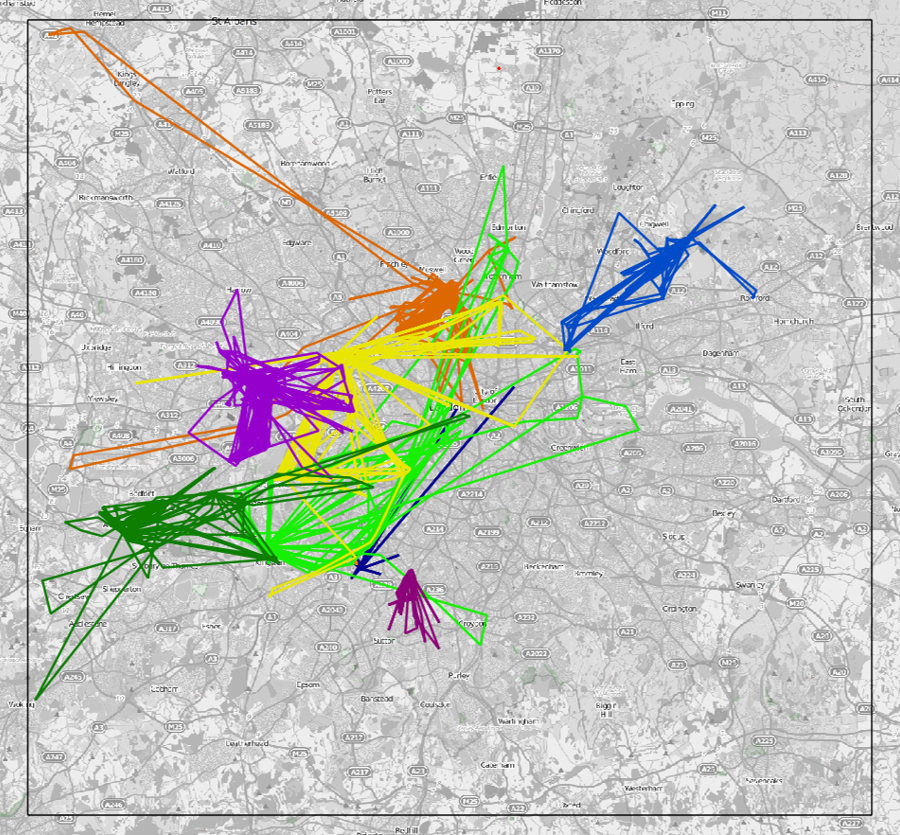
\includegraphics[width = 0.7\columnwidth]{figures/10_user_12_week_2-0_small.png}
		\subcaption{12-week trajectory of 10 users.}
    \label{fig:intro:10user}
	\end{subfigure}
  \caption{Illustration of Twitter Trajectories}\vspace{-0.0cm}
  \label{fig:exsinglefit}
	\figSpace
\end{figure}

In this work, the severity of privacy risks through publishing individual spatio-temporal data on the use case of Twitter data is investigated. In particular, it is shown that geotagged tweets might yield enough location information for building user specific trajectory profiles. Based on these profiles, Twitter accounts can be linked to additional trajectory data being observed from unknown users. Other location based services or mobile devices are also potential sources for trajectories. Additionally, face detection methods tag known persons in images in social networks. Thus, geotagged images can reveal a user's whereabouts at certain points in time. Given that there are multiple such images, it might be possible to build a trajectory and link it to a known user. To conclude, freely available location data might be used to link accounts and devices for the same user. Thus, the user reveals more of his movements and actions than might be intended.

To derive trajectory profiles for a given Twitter account, geotagged tweets containing an exact geolocation, a time, and a user ID were collected. Since this work focuses on the location aspect the content of the Tweet is completely ignored, even though it might add even more useful information to user profile. Using the Twitter API, or similar micro-blogging applications, users can publish a short text message, called a Tweet, together with their current geolocation, a current time-stamp, and their user ID.

The sequence of Tweets of a user is interpreted as a trajectory. For each user, all available Twitter data is used to build a trajectory profile to capture each user's specific mobility patterns. Using these profiles, new trajectories, for which the originating user is unknown, can be linked to a known user with an alarmingly high accuracy. To illustrate this classification problem, a typical Twitter trajectory of a single user is depicted in Figure \ref{fig:intro:1user}. The figure shows a twelve week trace of a user's tweets, in color-coded one-week intervals. For comparison, Figure \ref{fig:intro:10user} shows the same twelve week traces for ten users, using a different color per user. Note that the tweets of this user are voluntarily published by the user, such that Figure \ref{fig:intro:1user} and Figure \ref{fig:intro:10user} do not raise any privacy concerns.

The challenge of this work is to match a new short trajectory, such as a one week trajectory corresponding to a single color in Figure \ref{fig:intro:1user}, to the correct user corresponding to one of the colors in Figure \ref{fig:intro:10user}. Note that the ten selected user profiles in the example are located in  relatively distinct activity regions. Thus, finding the right profile is relatively simple. In a more realistic setting, distinguishing thousands of users in the same area, and user identification is significantly more challenging. In these experiments up to 15,989 users, within the same bounding box of London, are used leading to a much more challenging classification task.

Twitter data is comparatively sparse to other location tracking applications, as tweets are typically published at a frequency of less than one per hour. Despite this data sparsity, it is shown that a large quantity of low-quality location data can still be used to construct highly discriminative user models. To summarize the contributions of this work are as follows:

\begin{itemize}
	\item Trajectory models to capture user-specific movement profiles from sparse trajectories obtained from Twitter.
	\item Methods for mapping a newly observed trajectory of an unknown user to the most likely user in the database.
	\item An experimental evaluation showing that individual patterns are highly unique and allow for a user classification accuracy of up to 98\% .
	\item A case study of linking users of Twitter to users of Instagram, with an accuracy of up to $81\%$.
\end{itemize}

The remainder of this paper is organized as follows. Chapter~\ref{sec:rw} describes
related work of analyzing trajectory data and user identification. In Chapter~\ref{sec:probdef}, problem setting is formalized and the task of linking new trajectories to users is definied. Chapter~\ref{sec:method} describes the trajectory models and the approach to user identification. The results of the experimental evaluation are described in Chapter~\ref{sec:experiments}. Scalability of this solution is address in Chapter~\ref{sec:scalability} and further user linkage experiments are address in Chapter~\ref{sec:linkage}. It is concluded in Chapter~\ref{sec:conclusion}, with additional research opportunities addressed in Chapter~\ref{sec:additional}.
